\chapter{Fundamentação Teórica}

\section{Inversores de Fontes de Tensão}

\section{Modulação por Largura de Pulso - PWM}

A técnica de modulação por largura de pulso - PWM surge de problemáticas relacionadas ao controle da tensão de saída de inversores monofásicos, de forma contornar variações das tensões CC de entrada, regular a tensão dos inversores e cumprir os requisitos de controle de tensão e de frequência que devem permanecer constantes.

Dentre diversas técnicas empregadas para o controle de tensão, a modulação por largura de pulso senoidal (SPWM) é em geral mais empregada \cite{Rashid-Muhammad}.

\subsection{Modulação por Largura de Pulso Senoidal - SPWM}

A SPWM (do inglês \textit{Sinusoidal Pulse Width Modulation}), consiste na comparação de um sinal de referência senoidal com uma portadora triangular. Neste modelo de modulação, a frequência do sinal de referência $f_r$ determina a frequência do sinal de saída do inversor $f_o$. De forma similar, a amplitude de pico $A_r$ do sinal de referência controla o índice de modulação M e isso implica no controle da tensão RMS de saída $V_o$ do inversor. O índice de modulação M é dado pela Eq. (\ref{eq:indice_modulacao}), onde $V_{c}$ é a amplitude da onda portadora. A frequência da portadora normalizada é dada pela Eq. (\ref{eq:freq_portad_normaliz}), onde $f_c$ é a frequência da onda triangular.

\begin{align}
	M = \frac{V_r}{V_{c}} \label{eq:indice_modulacao} \\
	N = \frac{f_c}{f_r} \label{eq:freq_portad_normaliz}	
\end{align}

A comparação do sinal de referência $v_r$ com o sinal modulante $v_c$ gera uma saída em CA com valores de $V_i$ e $-V_i$. Desta forma, no estado 1, onde $v_r > v_c$, gera-se $V_i$ e no estado 2, onde $v_r < v_c$, gera-se $-V_i$. 

\section{Aquisição e Condicionamento de Sinais de Corrente e Tensão}

A etapa de aquisição e condicionamento de sinais destina-se à obtenção de tensões e correntes no ponto de conexão do inversor, e tem o objetivo entregar os parâmetros necessários para o algoritmo de controle realizado no microcontrolador. 

O sistema de aquisição e condicionamento de sinais é constituído pelos seguintes componentes:

\begin{itemize}
	\item Sensores de tensão e corrente;
	\item Filtros \textit{anti-aliasing};
	\item Circuitos de tratamento de sinal (somadores e reguladores de tensão)
\end{itemize}

\subsection{Transdutor de Tensão}

\subsection{Filtro Anti-Aliasing}

	Uma vez realizada a aquisição dos sinais de interesse, estes devem estar adequados para que sua manipulação por meio do microcontrolador seja possível. A rede elétrica possui diversos ruídos e transitórios eletromagnéticos de alta frequência que podem interferir no sinal de interesse (COLOCAR REFERÊNCIA), de modo que é necessário realizar uma filtragem analógica destas harmônicas indesejáveis anteriores ao microcontrolador.
	
	Desta forma, é utilizado na placa de aquisições um filtro \textit{butterworth} passa-baixas de 1ª ordem, com frequência de corte de 234 Hz. A topologia deste filtro é apresentada na Figura \ref{fig:filtro-butter}.
	
\begin{figure}[!hbt]
         % Center the figure.
         \begin{center}
         % Include the eps file, scale it such that it's width equals the column width. You can also put width=8cm for example...
         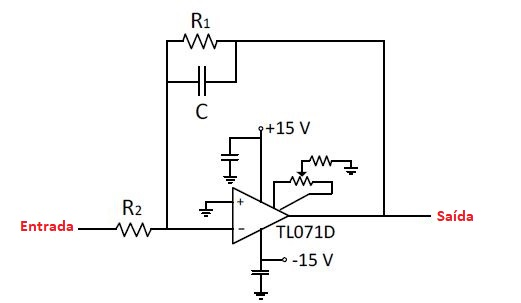
\includegraphics[scale=0.7]{figuras/filtro-butter.JPG}
         % Create a subtitle for the figure.
         \caption{Topologia do filtro de Butterworth de primeira ordem utilizado na placa de condicionamento de sinais}
         % Define the label of the figure. It's good to use 'fig:title', so you know that the label belongs to a figure.
         \label{fig:filtro-butter}
         \end{center}
 \end{figure}


	A frequência de corte deste filtro é dado pela Eq. 
	
\begin{align}
	f_{co} = \frac{1}{2\pi R_1 C} \label{eq:freq_corte_butter} \\
	K = -\frac{R_2}{R_1}\label{eq:ganho_butter}
\end{align}

\subsection{Circuito Somador}

Um circuito com amplificador operacional na topologia de somador é necessário para que se adicione um nível DC ao sinal proviniente do filtro \textit{anti-aliasing}, de forma que o sinal a ser amostrado reproduza apenas valores positivos e compatíveis com os limites de tensão do conversor A/D do microcontrolador. 

A topologia escolhida foi a de \textbf{somador não-inversor}, pois este não altera os ângulos de fase dos sinais provenientes dos transdutores. A Figura \ref{fig:somador-ninversor} mostra o circuito do somador não inversor. A equação que relaciona a tensão de saída com as tensões de entrada são dadas pela Eq. \ref{eq:circuito-somador}, onde $V_{REF}$ é a tensão de nível CC que é somada ao sinal que vem do filtro anti-aliasing, $V_1$.

\begin{align}
	V_{out} = \left(1+\frac{R_a}{R_b}\right)\left(\frac{V_1/R_1 + V_{REF}/R_2}{1/R_1 + 1/R_2}\right)\label{eq:circuito-somador}
\end{align}

\begin{figure}[!hbt]
	% Center the figure.
	\begin{center}
		% Include the eps file, scale it such that it's width equals the column width. You can also put width=8cm for example...
		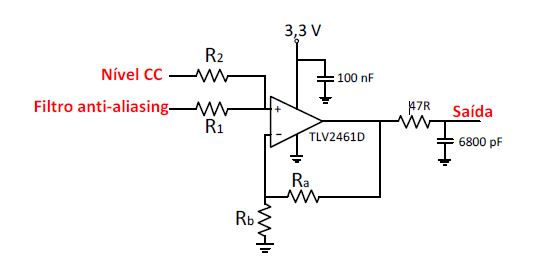
\includegraphics[scale=0.7]{figuras/somador-ninversor.JPG}
		% Create a subtitle for the figure.
		\caption{Circuito somador não-inversor}
		% Define the label of the figure. It's good to use 'fig:title', so you know that the label belongs to a figure.
		\label{fig:somador-ninversor}
	\end{center}
\end{figure}

\subsubsection{Circuito de fornecimento de tensão CC}

Um outro circuito, anterior ao somador é utilizado para fornecer tensão CC regulável ao somador, de forma que está possa estar dentro dos limites estabelecidos pelo microcontrolador. A Figura \ref{fig:divisor-tensao} mostra a topologia do circuito. A resistência variável conectada ao amplificador operacional permite o ajuste fino do divisor de tensão.

\begin{figure}[!hbt]
	% Center the figure.
	\begin{center}
		% Include the eps file, scale it such that it's width equals the column width. You can also put width=8cm for example...
		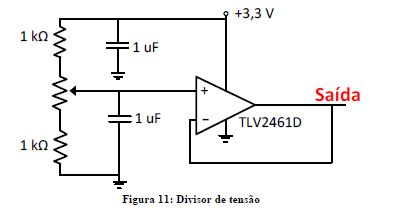
\includegraphics[scale=0.7]{figuras/divisor-tensao.JPG}
		% Create a subtitle for the figure.
		\caption{Divisor de tensão com resistência variável}
		% Define the label of the figure. It's good to use 'fig:title', so you know that the label belongs to a figure.
		\label{fig:divisor-tensao}
	\end{center}
\end{figure}

\subsection{Circuito Regulador de Tensão}

O circuito de regulação e filtragem de tensão destina-se ao suprimento de tensão aos amplificadores operacionais e transdutores da placa de aquisição. A Figura \ref{fig:circuito-regulacao} mostra os componentes deste circuito. Este é basicamente composto por \textit{beads} de ferrite e capacitores destinados à minimização de ruídos existentes na tensão de suprimento da placa. A placa de aquisição de sinais é alimentada por uma fonte externa que deve dispor de tensões contínuas de +15 V e -15 V.

\begin{figure}[!hbt]
	% Center the figure.
	\begin{center}
		% Include the eps file, scale it such that it's width equals the column width. You can also put width=8cm for example...
		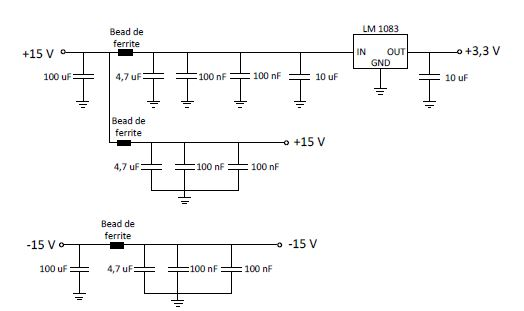
\includegraphics[scale=0.7]{figuras/circuito-regulador.JPG}
		% Create a subtitle for the figure.
		\caption{Circuito para regulação e filtragem de tensão}
		% Define the label of the figure. It's good to use 'fig:title', so you know that the label belongs to a figure.
		\label{fig:circuito-regulacao}
	\end{center}
\end{figure}


